\documentclass[12pt]{article}
\usepackage[utf8]{inputenc}
\usepackage{style}

\title{Oracle Quantum Computing}
\author{Joshua Spayd}
\date{\today}

\begin{document}
\maketitle

\section{Introduction}
It is the objective of the theoretical sciences to develop mathematical models
that describe natural phenomena, and when faced with a result that contradicts
existing models, it is the responsibility of the theorist to augment these
models to reconcile with the observed phenomena, and to resolve
inconsistencies across scientific theories. The strong Church-Turing thesis
conjectures that every physically realizable computation model can be
simulated by a Turing machine with polynomial overhead in runtime, but
physicist Richard Feynman \cite{Fey82} notes that the obvious classical
algorithm for simulating a quantum system of $n$ particles runs exponentially
in $n$ and suggests that computers be equipped with quantum mechanical gates
in order to enable efficient simulation of quantum systems. If quantum systems
cannot be efficiently simulated by Turing machines --- and if general-purpose
quantum computers are physically realizable --- then the strong Church-Turing
thesis is false, and we require a new model of computation. Though questions
of the feasibility and relative efficiency of quantum computers are yet
unanswered, this uncertainty has not prevented theorists from developing
quantum computational models. In this paper, we will formalize quantum computing
and quantum oracles, and then we will describe a few results from quantum
complexity theory, with emphasis on the result from \cite{BB92} that relative to
certain oracles, quantum computers are more powerful than nondeterministic
computers, or in the words of  Berthiaume and Brassard, that ``quantum can beat
nondeterminism.''


\section{Quantum mechanics}
\begin{figure}[H]
  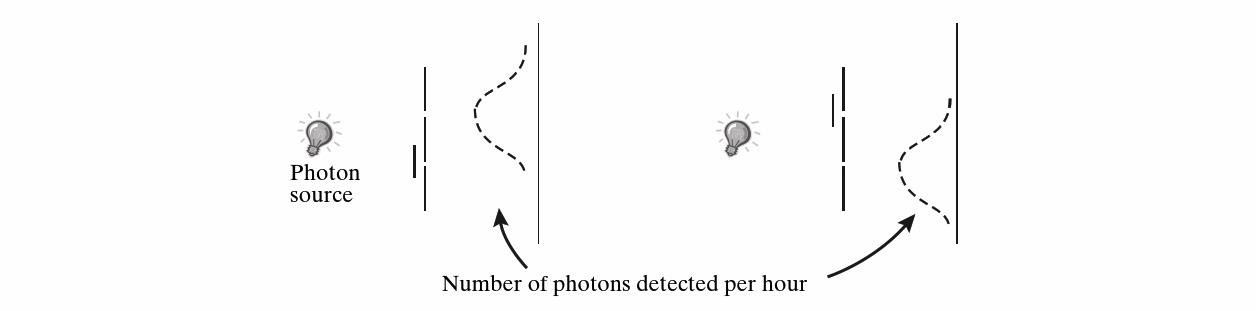
\includegraphics[width=\textwidth]{two-slit-1}
  \caption{\cite[p. 203]{AB09}}
  \label{fig:two-slit-1}
\end{figure}
\begin{figure}[H]
  
\includegraphics[width=\textwidth]{two-slit-2}
  \caption{\cite[p. 203]{AB09}}
  \label{fig:two-slit-2}
\end{figure}


\section{Modeling quantum computation}

\TODO{Mostly refer to {\cite{AB09}} here, maybe some {\cite{Wig19}}.}

\subsection{Quantum operations}

\subsection{Quantum Turing machines and the class $\BQP$}

\TODO{Define $\BQP$ and place it relative to $\BPP$ (theorem) and $\NP$
  (conjecture). Then describe what we will prove.}


\section{Quantum oracles}
\TODO{Refer to {\cite{BBBV97}}.}


\section{Quantum can beat nondeterminism \cite{BB92}}


\section{Further reading}


\nocite{*}
\bibliographystyle{alpha}
\bibliography{bibliography}
\end{document}
